\documentclass[11pt, a4paper]{article}
\usepackage[english]{babel}
\usepackage[utf8]{inputenc}
\usepackage{fancyhdr}
\usepackage{lastpage}
\usepackage{datetime}
\usepackage{indentfirst}
\usepackage{hyperref}
\usepackage{appendix}
\usepackage{amsmath}
\usepackage{amssymb}
\usepackage{amsfonts}
\usepackage{mathtools}
\usepackage{siunitx}
\usepackage{cancel}
\usepackage{tabularray}
\usepackage{multirow}
\usepackage{array}
\usepackage{hhline}
\usepackage{makecell}
\usepackage{courier}
\usepackage[font=small, skip=0pt]{caption}
\usepackage[font=scriptsize, skip=0pt]{subcaption}
\usepackage{float}
\usepackage{graphicx}
\usepackage{listings}
\usepackage{xcolor}
\usepackage{matlab-prettifier}
\usepackage[T1]{fontenc}
\usepackage{lmodern}
\usepackage{bigfoot}
\usepackage{filecontents}
\usepackage[nottoc]{tocbibind}

\graphicspath{ {./mathimages/} }

\newdateformat{Datea}{\THEDAY\ \monthname[\THEMONTH] \THEYEAR}
\newdateformat{Dateb}{\monthname[\THEMONTH] \THEYEAR}

%\allowdisplaybreaks
\DeclareMathOperator{\cosec}{cosec}
\DeclareMathOperator{\cotan}{cotan}
\DeclareMathOperator{\sech}{sech}
\DeclareMathOperator{\cosech}{cosech}
\DeclareMathOperator{\arcsec}{arcsec}
\DeclareMathOperator{\arccot}{arccot}
\DeclareMathOperator{\arccsc}{arccosec}
\DeclareMathOperator{\arccosh}{arccosh}
\DeclareMathOperator{\arcsinh}{arcsinh}
\DeclareMathOperator{\arctanh}{arctanh}
\DeclareMathOperator{\arcsech}{arcsech}
\DeclareMathOperator{\arccsch}{arccsch}
\DeclareMathOperator{\arccoth}{arccoth}
\DeclareMathOperator{\arsinh}{arsinh}
\DeclareMathOperator{\arcosh}{arcosh}
\DeclareMathOperator{\artanh}{artanh}

\DeclareMathOperator{\cis}{cis}

\pagestyle{fancy}
\fancyhf{}
\rhead{Hatam Barma}
\chead{\begin{tabular}[t]{@{}l@{}}\\Mathematics and Further Mathematics Pure Revision Summary\end{tabular}}
\lhead{\Dateb\today}
\cfoot{Page \thepage}

\renewcommand{\thesection}{\arabic{section}} 

\renewcommand{\thesubsection}{\thesection.\arabic{subsection}}

\setcounter{section}{2}

\allowdisplaybreaks

\fancypagestyle{plain}{
\fancyhf{}
\renewcommand{\headrulewidth}{0pt}}

\hypersetup{
    colorlinks,
    citecolor=black,
    filecolor=black,
    linkcolor=blue,
    urlcolor=magenta!70!black
}

\begin{document}


\begin{titlepage}
   \begin{center}
       \vspace*{2.5cm}
	\huge
       \textbf{A-Level Mathematics and Further Mathematics Pure Revision Summary} \\
	\vspace{1cm}
	\Large
       \textbf{Chapter 3: Calculus II: Integration}
            
       \vspace{1.5cm}
	\LARGE
       \textbf{Hatam Barma} \\
	\vspace{0.75cm}
       \normalsize
       \emph{Compiled on \Datea\today} \\

       \vfill
        

	E-mail: hatam.barma@gmail.com
   \end{center}
\end{titlepage}


\tableofcontents

\clearpage
\section{Calculus II: Integration}
\vspace{0.5cm}

\subsection{Anti-differentiation}
\begin{itemize}
\item A Level M AS / Year 1 \hspace{1cm} \phantom{ } Pages 291 -- 300
\end{itemize} \par
Anti-differentiation is the act of taking a function and finding a function which gives your starting function as a derivative. For example: 
\begin{flalign*}
\frac{\mathrm{d}y}{\mathrm{d}x}=x^{n} \;\Longleftrightarrow\; y=\frac{1}{n+1}x^{n+1}+c \hspace{1.75cm} \text{where }c\text{ is any intercept} &&
\end{flalign*}
We use the integral sign, $\int$ to denote an anti-derivative.
\begin{flalign*}
&\int f(x)+g(x)\, \mathrm{d}x=\int f(x)\, \mathrm{d}x+\int g(x)\, \mathrm{d}x && \\
&\int k\cdot f(x)\, \mathrm{d}x=k\cdot\int f(x)\,\mathrm{d}x &&\\
&\int 3x^{4}-x^{-2}\,\mathrm{d}x=\frac{3}{5}x^{5}+x^{-1}+c && \\
&\int x^{n}\,\mathrm{d}x =\frac{1}{n+1}x^{n+1}+c \hspace{2.75cm} (n\neq 1) && \\
\end{flalign*}
While this is trivial for simple functions, such as polynomials (as above), there are various other methods that can be used, which are detailed in subsequent sections. The list of useful derivatives in section \ref{usefulderivatives} will continue to be useful for anti-differentiation / integration.
\vspace{0.5cm}


\subsection{Integration}
\begin{itemize}
\item A Level M AS / Year 1 \hspace{1cm} \phantom{ } Pages 291 -- 310
\item A Level M Year 2 \hspace{1cm} \phantom{ AS / } Pages 269 -- 277
\end{itemize} \par
Integration is anti-differentiation of specific areas. When evaluated with limits, it calculates the \emph{signed area}. If the curve goes below the $x$-axis, the area is evaluated as negative. When integrating the area  between two curves, find the area beneath each curve, and subtract from one another, or do the single integral of $(\int\left[\mathrm{Top\,-\,Bottom}\right]\,\mathrm{d}x)$

\scriptsize
\begin{flalign*}
\int_{0.5}^{2}-x^{2}+2x+3\,\mathrm{d}x &= \left[ -\frac{x^{3}}{3}+x^{2}+3x\, (+c) \right]_{0.5}^{2} && \\
&=\left[ -\frac{(2)^{3}}{3}+(2)^{2}+3(2)\, (+c) \right]-\left[ -\frac{(0.5)^{3}}{3}+(0.5)^{2}+3(0.5)\, (+c) \right] && \\
&=\frac{45}{8}+\left[ c-c \right] \hspace{1.5cm} \text{The $c$ terms cancel, so not necessary to include}
\end{flalign*}
\normalsize
\vspace{0.3cm}


\subsection{Integration by inspection}
\begin{itemize}
\item A Level M Year 2 \hspace{1cm} \phantom{ AS / } Pages 219 -- 223
\end{itemize}
If you are lucky, you may be able to spot the impact of a chain rule on an integrand, and so can give a good guess as to the result of the integral. For example
\begin{equation*}
\int \frac{x}{x^{2}+1}\,\mathrm{d}x=\frac{1}{2}\ln\left( x^{2}+1 \right)+c
\end{equation*}
Since by use of the chain rule, the derivative of the argument of $\ln$ is a factor of the numerator of the fraction. A further example is
\begin{equation*}
\int \tan(x)\,\mathrm{d}x=\int \frac{\sin(x)}{\cos(x)}\,\mathrm{d}x=-\ln(\cos(x))
\end{equation*}
As the derivative of $\cos(x)$ is $\sin(x)$ which appears in the numerator.
\vspace{0.5cm}


\subsection{Integration by parts}
\begin{itemize}
\item A Level M Year 2 \hspace{1cm} \phantom{ AS / } Pages 230 -- 234
\end{itemize} \par
This method is useful when evaluating the integral of product of two functions. Assuming the function $f(x)$ can be re-written as $u(x)\times\frac{\mathrm{d}v}{\mathrm{d}x}$. Then by using the results of the product rule, it converts the integral into a form that \emph{may} be easier to solve. 
\small
\begin{flalign*}
\frac{\mathrm{d}}{\mathrm{d}x}\left[ u(x)\cdot v(x) \right]&=u(x)\times\frac{\mathrm{d}v}{\mathrm{d}x}+\frac{\mathrm{d}u}{\mathrm{d}x}\times v(x)  \hspace{1cm} \text{Take anti-derivative of both sides}&&\\
u(x)\cdot v(x)&=\int\,\left[ u(x)\times\frac{\mathrm{d}v}{\mathrm{d}x}+\frac{\mathrm{d}u}{\mathrm{d}x}\times v(x) \right]\mathrm{d}x&&\\
&=\int\,\left[ u(x)\times\frac{\mathrm{d}v}{\mathrm{d}x} \right] \mathrm{d}x+\int \left[ \frac{\mathrm{d}u}{\mathrm{d}x}\times v(x) \right]\mathrm{d}x
\end{flalign*}\\ \normalsize
Therefore, integration by parts can be expressed as:
\begin{equation*}
\int u(x)\times \frac{\mathrm{d}v}{\mathrm{d}x}\,\mathrm{d}x=u(x)\cdot v(x)-\int v(x)\times \frac{\mathrm{d}u}{\mathrm{d}x} \, \mathrm{d}x
\end{equation*} \\
Or, when evaluated with limits;
\begin{equation*}
\int_{a}^{b} u(x)\times \frac{\mathrm{d}v}{\mathrm{d}x}\,\mathrm{d}x=\left[ u(x)\cdot v(x) \right] _{a}^{b}-\int_{a}^{b} v(x)\times \frac{\mathrm{d}u}{\mathrm{d}x} \, \mathrm{d}x
\end{equation*}

How do you decide which part of the integrand to be $u$, and which to be $\frac{\mathrm{d}v}{\mathrm{d}x}$? The acronym `\emph{LIATE}' can help pick a `$u$' function. If any component of the integrand is one of the following, then this should be chosen to be the `$u$' function, with priority given to logarithms, then inverse trigonometrics, etc.
\begin{center}
\begin{tblr}{|[.75pt]|c|l|l||[.75pt]}
\hline[.75pt]
\emph{L} & Logarithm & i.e. $\ln{(x)}$, $\log{(x)}$ \\ \hline
\emph{I} & Inverse trigonometric & i.e. $\arcsin(x)$, $\arccos(x)$ \\ \hline
\emph{A} & Algebraic & i.e. $3x^{2}+1$, polynomials \\ \hline
\emph{T} & Trigonometric & i.e. $\tan(x)$, $\sin(x)$ \\ \hline
\emph{E} & Exponential & i.e. $e^{x}$, $\sinh(x)$ \\ \hline[.75pt]
\end{tblr}
\end{center}
\vspace{0.5cm}

\subsection{Integration by substitution}
\begin{itemize}
\item A Level M Year 2 \hspace{1cm} \phantom{ AS / } Pages 223 -- 230
\end{itemize} \par
This involves making a substitution for $x$ which makes the integral easier to solve. For example, the substitution $u=3x-2$ makes the following integral considerably easier to solve:
\begin{equation*}
\int_{2}^{3}x\sqrt{3x-2}\,\mathrm{d}x=\int_{4}^{7}\frac{(u+2)}{3}\sqrt{u}\times\frac{\mathrm{d}x}{\mathrm{d}u}\,\mathrm{d}u
\end{equation*}
\emph{Note: The limits must be changed too, to be consistent with the substitution} \newline \par
Since the scale of the axis is different, the correction factor is $\frac{\mathrm{d}x}{\mathrm{d}u}$ This can be thought of as the two $\mathrm{d}u$ terms cancelling, leaving the integration with respect to $x$. \newline \par
When performing an \emph{indefinite integral}, the result comes out in terms of $u$, so $x$ must be substituted back into the result. A definite integral does not need this, since the limits are also changed according to the substitution. Section \ref{usefulintegrals} contains some useful integral substitutions. 
\vspace{0.5cm}


\subsection{Standard integrals}
\label{usefulintegrals}
\begin{itemize}
\item A Level FM Year 2 \hspace{1cm} \phantom{AS /} Pages 157 -- 163
\end{itemize} \par
Here are some integrals which substitutions make considerably simpler. These are \underline{all} in the formula booklet, so while it is good to recognise them, there is no need to memorise the substitutions required in each case.

\begin{center}
\begin{tblr}{|[.75pt]|c|c||[.75pt]}
\hline[1.25pt]
$f(x)$ & $\int f(x)\,\mathrm{d}x$ \\ \hline[.75pt]
$\frac{1}{\sqrt{a^{2}-x^{2}}}$ & $\sin^{-1}\left(\frac{x}{a}  \right)$ for $\left( |x|<a \right)$ \\ \hline
$\frac{1}{a^{2}+x^{2}}$ & $\frac{1}{a}\tan^{-1}\left(\frac{x}{a}  \right)$  \\ \hline
$\frac{1}{\sqrt{a^{2}-x^{2}}}$ & $\sinh^{-1}\left(\frac{x}{a}  \right)$ or $\ln\left( x+\sqrt{x^{2}+a^{2}} \right)$  \\ \hline
$\frac{1}{\sqrt{x^{2}-a^{2}}}$ & $\cosh^{-1}\left(\frac{x}{a}  \right)$ or $\ln\left( x+\sqrt{x^{2}-a^{2}} \right)$ for $x>a$  \\ \hline[.75pt]
\end{tblr}
\end{center}
\vspace{0.5cm}


\subsection{Integration by partial fractions}
\begin{itemize}
\item A Level M Year 2 \hspace{1cm} \phantom{ AS / } Pages 239 -- 243
\item A Level FM Year 2 \hspace{1cm} \phantom{AS /} Pages 163 -- 166
\end{itemize} \par
Rational functions, for example $\frac{7x+4}{(x+2)(2x-1)}$ can be re-written in partial fractions (see sections \ref{partialfractions1} and \ref{partialfractions2} for more on how to do this). In this case, it decomposes into $\frac{2}{x+2}+\frac{3}{2x-1}$. This \emph{may} make the integration of a rational function easier.
\vspace{0.5cm}


\subsection{Improper integrals}
\begin{itemize}
\item A Level FM Year 2 \hspace{1cm} \phantom{AS /} Pages 179 -- 183
\end{itemize} \par
Some functions are undefined at certain points (i.e $\frac{1}{1-x}$ is undefined at $x=1$) and so the integral is undefined too; other integrals are over an infinite range, and so these integrals are called \emph{improper}.

\begin{flalign*}
&\int_{0}^{\infty}e^{-3x}\,\mathrm{d}x &&\text{is improper because the range of integration is infinite} && \\
&\int_{0}^{3}\frac{1}{\sqrt{3-x}}\,\mathrm{d}x &&\text{is improper because the integrand is undefined at $x=3$} && \\
&\int_{1}^{\infty} \frac{1}{x}\,\mathrm{d}x &&\text{is improper because the range of integration is infinite} &&
\end{flalign*}

We can deal with these types of integrals by setting the undefined integral limit to a variable (let us say $b$ in this case), and then take the limit as $b$ tends to the indeterminate limit. This is best illustrated by an example:
\newpage
\begin{flalign*}
\int_{0}^{\infty}e^{-3x}\,\mathrm{d}x &= \lim_{b \to \infty}\left[ \int_{0}^{b}e^{-3x}\,\mathrm{d}x \right] && \\
&=\lim_{b\to\infty}\left[ \left[ -\frac{1}{3}e^{-3x}\right]_{0}^{b}\right] && \\
&=\lim_{b\to\infty}\left[ -\frac{1}{3}e^{-3b}--\frac{1}{3}e^{0} \right] && \\
&=\lim_{b\to\infty}\left[-\frac{1}{2}e^{-3b}+\frac{1}{3}\right] &&
\end{flalign*}
And as $b\rightarrow\infty$, $-\frac{1}{3}e^{-3b}\rightarrow0$, so $\int_{0}^{\infty}e^{-3x}\,\mathrm{d}x=\frac{1}{3}$\\
Therefore the integral  $\int_{0}^{\infty}e^{-3x}\,\mathrm{d}x$ \emph{does} exist, or converges, and has value $\frac{1}{3}$ \newline \par

\begin{flalign*}
\int_{0}^{3}\frac{1}{\sqrt{3-x}}\,\mathrm{d}x &= \lim_{b \to 3}\left[ \int_{0}^{3}\frac{1}{\sqrt{3-x}}\,\mathrm{d}x \right] && \\
&=\lim_{b\to3}\left[ \left[ -2\sqrt{3-x}\right]_{0}^{b}\right] && \\
&=\lim_{b\to3}\left[ \left[ -2\sqrt{3-b} - -2\sqrt{3-0}\right]_{0}^{b}\right] && \\
&=2\sqrt{3} &&
\end{flalign*}
Therefore the integral  $\int_{0}^{3}\frac{1}{\sqrt{3-x}}\,\mathrm{d}x$ \emph{does} exist, or converges, and has value $2\sqrt{3}$ \newline \par

\begin{flalign*}
\int_{0}^{\infty}\frac{1}{x}\,\mathrm{d}x &= \lim_{b\to\infty}\left[ \left[ \ln(x)\right]_{0}^{b}\right] && \\
&=\lim_{b\to\infty}\left[ \ln(b)-\ln(0) \right] && \\
&=\lim_{b\to\infty}\left[-\frac{1}{2}e^{-3b}+\frac{1}{3}\right] &&
\end{flalign*}
However as $b\rightarrow\infty$, $\ln(b)\rightarrow\infty$, so $\int_{0}^{\infty}\frac{1}{x}\,\mathrm{d}x$ is not defined.\\
\begin{itemize}
\item[Note:] If the integrand is undefined between the limits, we must evaluate the integral between each of the limits and the point at which it is undefined.
\end{itemize}
\vspace{0.5cm}

\subsection{Polar integration}
\begin{itemize}
\item A Level FM Year 2 \hspace{1cm} \phantom{AS /} Pages 210 -- 216
\end{itemize} \par
\begin{figure}[H]
\centering
\begin{subfigure}[b]{0.49\textwidth}
Polar integration measures the area `swept out' by the curve, as opposed to the area directly beneath it. \newline \par

We can use a triangle approximation, whereby:
\vspace{-0.2cm}
\begin{equation*}
\text{Area of a triangle}=\frac{1}{2}ab\sin(C)
\end{equation*}
\end{subfigure}
\hfill
\begin{subfigure}[b]{0.49\textwidth}
\centering
\scalebox{.85}{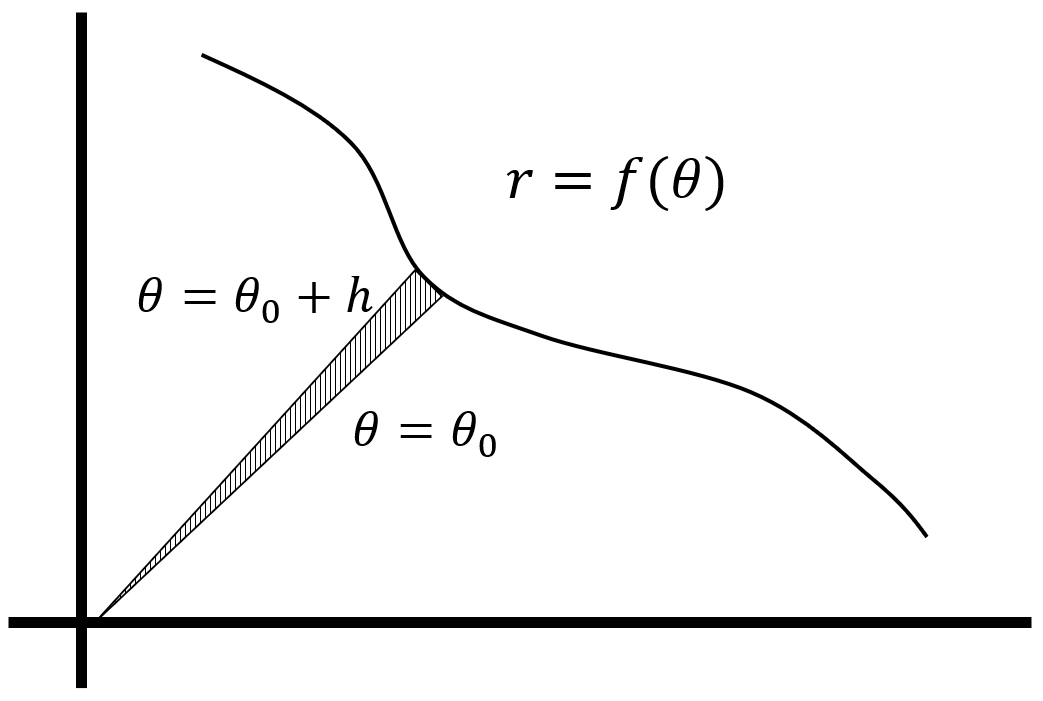
\includegraphics[width=\textwidth]{polarintegration}}
\end{subfigure}
\end{figure}
So, the area swept out by the triangle is:
\begin{flalign*}
&=\lim_{h\to0}\left[ \frac{1}{2}\times f(\theta_{0})\times f(\theta_{0}+h)\times\sin(h) \right] && \\
&\textcolor{white}{=\;\;}f(\theta_{0}+h)\rightarrow f(\theta_{0})\text{ and }\sin(h)\rightarrow h\text{, so} &&\\
&=\frac{1}{2}\times f(\theta_{0})^{2}\times h &&
\end{flalign*}
The area swept out by the curve is then the sum of the triangles.
\begin{flalign*}
Area&=\sum triangles &&=\sum \frac{1}{2}f(\theta_{0})^{2}h &&=\int\frac{1}{2}f(\theta_{0})^{2}\,\mathrm{d}\theta &&\\
&&\\
Area&=\int\frac{1}{2}r^{2}\,\mathrm{d}\theta &&
\end{flalign*}
\vspace{0.5cm}


\subsection{The Trapezium Rule}
\begin{itemize}
\item A Level M Year 2 \hspace{1cm} \phantom{ AS / } Pages 331 -- 341
\end{itemize} \par
In order to estimate the area of a curve without integrating, the area can be approximated by summing a series of trapezia between the limits. The number of divisions between the limits determines the accuracy of the approximation. 
\begin{figure}[H]
\centering
\begin{subfigure}[b]{0.49\textwidth}
\centering
\scalebox{1.2}{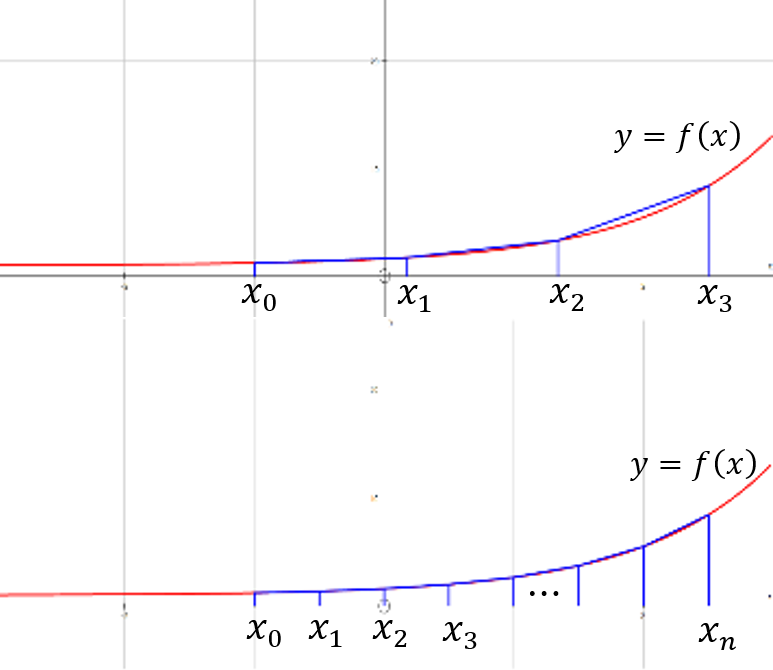
\includegraphics[width=\textwidth]{trapeziumrule}}
\end{subfigure}
\end{figure}
\noindent So, this approximate sum can be written as:
\begin{flalign*}
\int_{x_{0}}^{x^{n}}f(x)\,\mathrm{d}x&=\sum_{k=0}^{n-1}\left[ \left( y_{k}+y_{k+1}\right)\times\frac{h}{2} \right] && \\
\int_{x_{0}}^{x^{n}}f(x)\,\mathrm{d}x&=\frac{h}{2}\left[ y_{0}+2\left( y_{1}+y_{2}+\cdots+y_{n-2}+y_{n-1}\right)+y_{n}\right] &&
\end{flalign*}
\vspace{0.5cm}


\subsection{Parametric integration}
\begin{itemize}
\item A Level M Year 2 \hspace{1cm} \phantom{ AS / } Pages 263 -- 265
\end{itemize} \par
Used to integrate a curve given by a set of parametric equations, where the limits may be given in terms of the additional parameter, $t$, as opposed to in terms of $x$.
\begin{figure}[H]
\centering
\begin{subfigure}[b]{0.39\textwidth}
\begin{flalign*}
&\begin{Bmatrix}x=f(t) \\ y=g(t)\end{Bmatrix} \Rightarrow \frac{\mathrm{d}y}{\mathrm{d}x}=\frac{\left(\frac{\mathrm{d}y}{\mathrm{d}t}\right)}{\left(\frac{\mathrm{d}x}{\mathrm{d}t}\right)} &&\\
&&\\
&\int_{a}^{b}y\,\mathrm{d}x=\int_{t=t_{0}}^{t=t_{1}}y\frac{\mathrm{d}x}{\mathrm{d}t}\,\mathrm{d}t &&\\
&&
\end{flalign*}
\end{subfigure}
\hfill
\begin{subfigure}[b]{0.59\textwidth}
\centering
\scalebox{1}{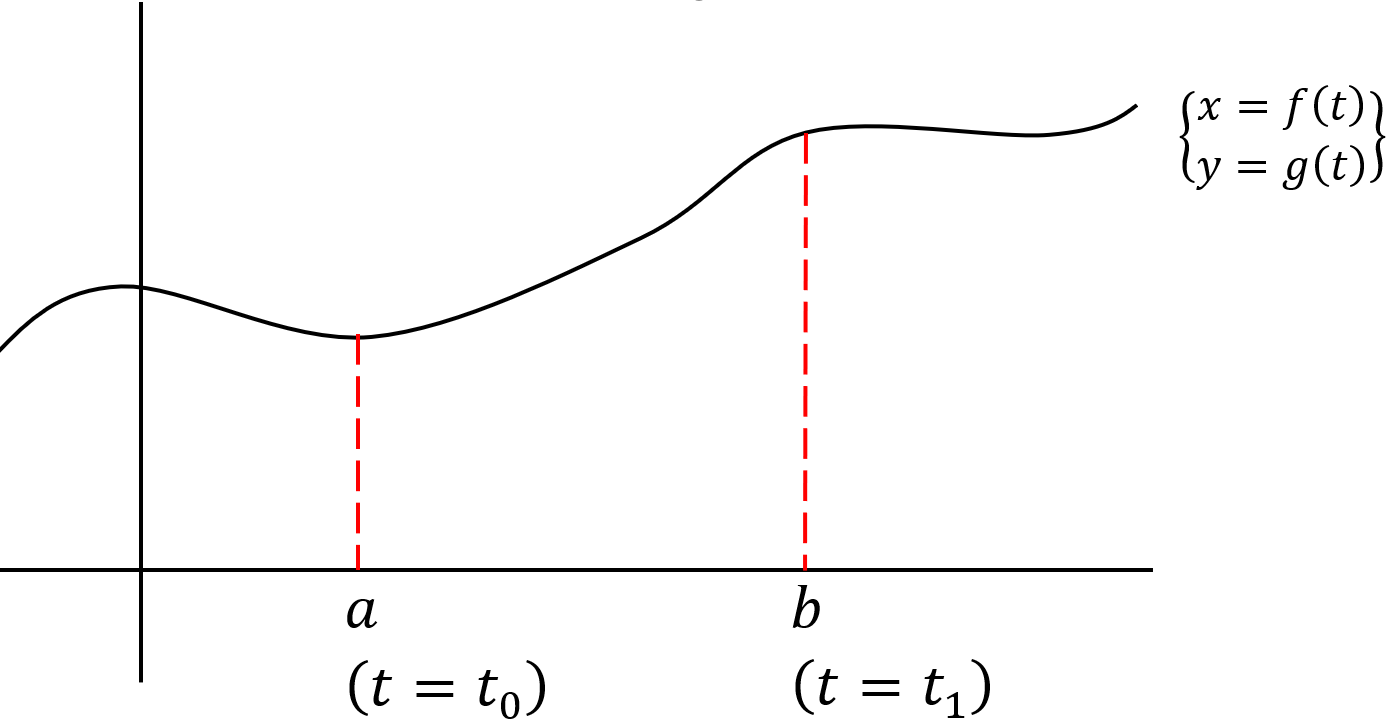
\includegraphics[width=\textwidth]{parametricintegration}}
\end{subfigure}
\end{figure}
\vspace{0.5cm}


\subsection{Volumes of revolution}
\begin{itemize}
\item A Level FM Year 2 \hspace{1cm} \phantom{AS /} Pages 183 -- 190
\end{itemize} \par
A volume of revolution is the volume obtained by rotating a curve around an axis, and then taking the volume enclosed by the surface created.
\begin{figure}[H]
\centering
\begin{subfigure}[b]{0.59\textwidth}
When we calculate a definite integral, one way of thinking about it is summing up the areas of infinitely small rectangles. Therefore when we calculate a volume of revolution, we can consider it to be a sum of the volumes of infinitely thin cylinders. \newline \par
\end{subfigure}
\hfill
\begin{subfigure}[b]{0.39\textwidth}
\centering
\scalebox{1}{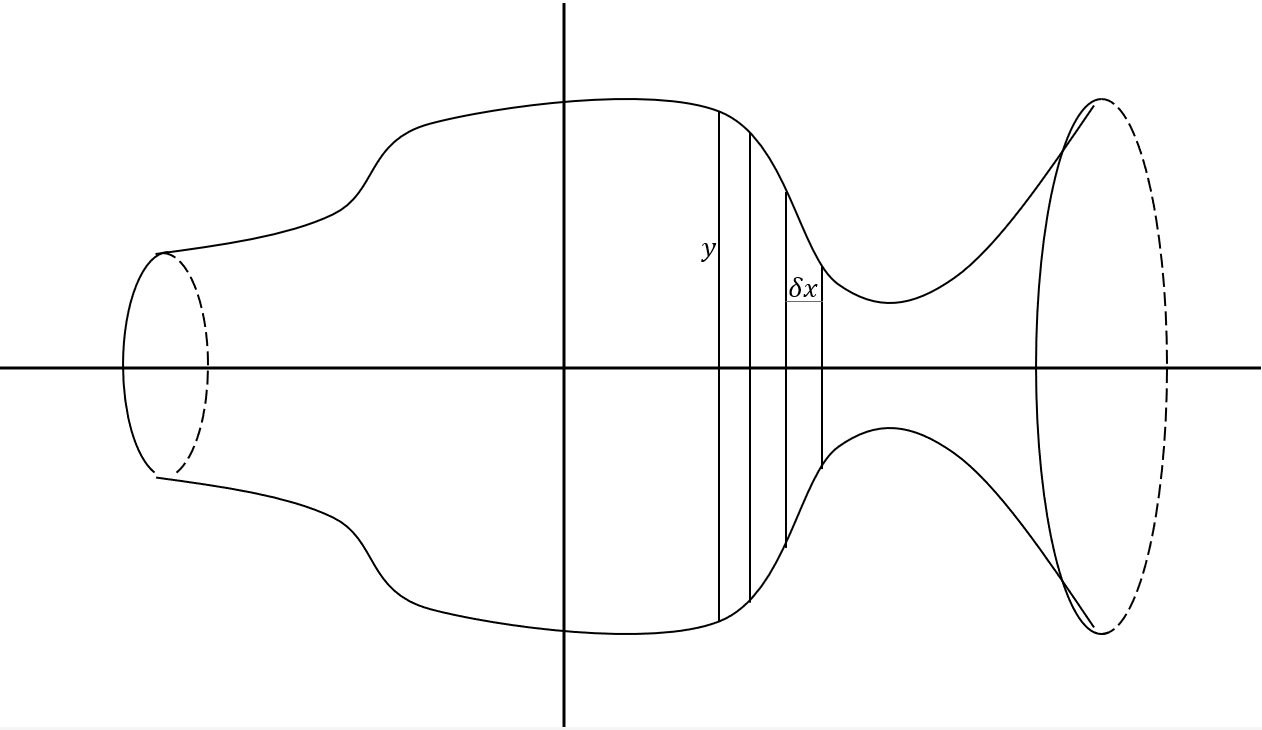
\includegraphics[width=\textwidth]{volumesofrevolution1}}
\end{subfigure}
\end{figure}
\noindent The volume of each cylinder is $V_{\text{cylinder}}=\pi r^{2}h$, where:\\
The radius, $r$, is the height of the curve at theat point, ($r=y$) \\
The height, $h$, is the width of each cylinder $\delta x$ \\
\begin{flalign*}
\text{So }V_{\text{cylinder}}&=\pi y^{2} \delta x & &&\\
\text{So }V_{\text{Total}}&=\sum V_{\text{cylinders}} && \\
&=\sum \pi y^{2} \delta x  & \text{As $\delta x \rightarrow 0$, becomes an infinitessimal sum}&& \\
&=\int\pi y^{2}\,\mathrm{d}x &&
\end{flalign*}
If doing this with parametric equations,
\begin{equation*}
V_{\text{Total}}=\int\pi\cdot y(t)^{2}\cdot\frac{\mathrm{d}x}{\mathrm{d}t}\,\mathrm{d}t
\end{equation*}

If rotating about the $y$-axis, then all the $x$ terms are swapped with $y$ terms.

\vspace{0.5cm}
\end{document}